\documentclass[11pt]{article}
\usepackage{graphicx}
\usepackage{enumitem}
\usepackage{lipsum}

%\usepackage{subfig}


%%%%%%%%%%%%%%%%%%%%%%%%%%%%%%%%%%%%%%%%%%%%%%%%%%%%%%%%%%%%%%%%%%%%%%%%%%%%%%%%
% packages
%%%%%%%%%%%%%%%%%%%%%%%%%%%%%%%%%%%%%%%%%%%%%%%%%%%%%%%%%%%%%%%%%%%%%%%%%%%%%%%%

\usepackage{coling2020}
\usepackage{times}
\usepackage{url}
\usepackage{amsmath,amsfonts}
\usepackage{latexsym}
\usepackage{hyperref}
\hypersetup{
  colorlinks   = true, %Colours links instead of ugly boxes
  urlcolor     = blue, %Colour for external hyperlinks
  linkcolor    = blue, %Colour of internal links
  citecolor    = blue  %Colour of citations
}
\usepackage{CJKutf8}
\usepackage{subfig}
\usepackage[sort&compress,round,comma,authoryear]{natbib}

\usepackage{csquotes}
\renewcommand{\mkbegdispquote}[2]{\itshape}

%%%%%%%%%%%%%%%%%%%%%%%%%%%%%%%%%%%%%%%%%%%%%%%%%%%%%%%%%%%%%%%%%%%%%%%%%%%%%%%%
% latex functions
%%%%%%%%%%%%%%%%%%%%%%%%%%%%%%%%%%%%%%%%%%%%%%%%%%%%%%%%%%%%%%%%%%%%%%%%%%%%%%%%

\newcommand{\ltwo}[1]{\lVert{#1}\rVert}
\newcommand{\indicator}[1]{\mathbbm{1}\!\left[{#1}\right]}
\newcommand{\R}{\mathbb R}
\newcommand{\TEXT}{\texttt{text}}

\newcommand{\defn}[1]{\emph{{#1}}}
\newcommand{\fixme}[1]{{\color{red} \textbf{FIXME:} {\textit {#1}}}}
%\newcommand{\fixme}[1]{}
\newcommand{\XXX}{{\textbf{XXX}}~}
\newcommand{\bertmoji}{\texttt{BERTmoticon}}
\newcommand{\bertmojill}{\texttt{BERTmoticon-LL}}
%\newcommand{\bert}{\texttt{BERT-multilingual}}
\newcommand{\bert}{\text{multilingual BERT}}

\DeclareMathOperator*{\argmax}{arg\,max}
\DeclareMathOperator*{\argmin}{arg\,min}
\DeclareMathOperator{\acc}{acc}
\DeclareMathOperator{\none}{\texttt{None}}
%\DeclareMathOperator{\model}{\texttt{BERTMultilingualEmoticon}}
\DeclareMathOperator{\emoticon}{\texttt{TwitterEmoticon}}
\DeclareMathOperator{\emoticonTrain}{\texttt{TwitterEmoticon\_train}}
\DeclareMathOperator{\emoticonValid}{\texttt{TwitterEmoticon\_valid}}
\DeclareMathOperator{\emoticonTest}{\texttt{TwitterEmoticon\_test}}
\DeclareMathOperator{\corona}{\texttt{TwitterCorona}}

%%%%%%%%%%%%%%%%%%%%%%%%%%%%%%%%%%%%%%%%%%%%%%%%%%%%%%%%%%%%%%%%%%%%%%%%%%%%%%%%
% paper configuration
%%%%%%%%%%%%%%%%%%%%%%%%%%%%%%%%%%%%%%%%%%%%%%%%%%%%%%%%%%%%%%%%%%%%%%%%%%%%%%%%

%\setlength\titlebox{5cm}
%\colingfinalcopy % Uncomment this line for the final submission

% You can expand the titlebox if you need extra space
% to show all the authors. Please do not make the titlebox
% smaller than 5cm (the original size); we will check this
% in the camera-ready version and ask you to change it back.


%\title{$\bertmoji$ says: "wear a mask" :  
\includegraphics[scale=0.07]{images/mask_photo.png}}
\title{Multilingual Emoticon Prediction of Tweets about COVID-19 
\includegraphics[height=0.8em]{images/mask_photo.png}}

\author{First Author \\
  Affiliation / Address line 1 \\
  Affiliation / Address line 2 \\
  Affiliation / Address line 3 \\
  {\tt email@domain} \\\And
  Second Author \\
  Affiliation / Address line 1 \\
  Affiliation / Address line 2 \\
  Affiliation / Address line 3 \\
  {\tt email@domain} \\}

\date{}

%%%%%%%%%%%%%%%%%%%%%%%%%%%%%%%%%%%%%%%%%%%%%%%%%%%%%%%%%%%%%%%%%%%%%%%%%%%%%%%%
% document text
%%%%%%%%%%%%%%%%%%%%%%%%%%%%%%%%%%%%%%%%%%%%%%%%%%%%%%%%%%%%%%%%%%%%%%%%%%%%%%%%

\begin{document}
\maketitle
\begin{abstract}
    %There are no multi-lingual emoji prediction models. This makes it hard to investigate
    %how different languages use emojis. We present $\bertmoji$, a multi-lingual model 
    %that fine tunes the \texttt{BERTMultilingual} to the emoji prediction task.
    Emojis are a widely used tool for encoding emotional content in informal messages such as tweets,
    and predicting which emoji corresponds to a piece of text can be used as a proxy for measuring the emotional content in the text.
    This paper presents the first model for predicting emojis in highly multilingual text.
    Our $\bertmoji$ model is a fine-tuned version of the $\bert$ model,
    and it can predict emojis for text written in 102 different languages.
    We trained our $\bertmoji$ model on 54.2 million geolocated tweets sent in the first 6 months of 2020,
    and we apply the model to a case study analyzing the emotional reaction of Twitter users to news about the coronavirus.
    Example findings include a spike in sadness when the World Health Organization (WHO) declared that coronavirus was a global pandemic,
    and a spike in anger and disgust when the number of COVID-19 related deaths in the United States surpassed one hundred thousand.
    We provide an easy-to-use and open source python library for predicting emojis with $\bertmoji$ so that the model can easily be applied to other data mining tasks.
    %\fixme{
    %For example, when the World Health Organization (WHO) declared that coronavirus was a global pandemic on \XXX,
    %we observe a spike in sadness and a decrease in fear.
    %We further observe that the mask emoji \XXX is highly correlated with \XXX.
%}
    %We achieve an F1-score of 21\% across the different languages and by applying this model to the coronavirus responses and mapping those emoji response to the Plutchik wheel; we tapped into the peoples' sentiment throughout the COVID-19 timeline. 
    %\fixme{Add a 1 sentence summary of the results?}
\end{abstract}

%
% The following footnote without marker is needed for the camera-ready
% version of the paper.
% Comment out the instructions (first text) and uncomment the 8 lines
% under "final paper" for your variant of English.
% 
\blfootnote{
    %
    % for review submission
    %
    \hspace{-0.65cm}  % space normally used by the marker
    Place licence statement here for the camera-ready version. 
    %
    % % final paper: en-uk version 
    %
    % \hspace{-0.65cm}  % space normally used by the marker
    % This work is licensed under a Creative Commons 
    % Attribution 4.0 International Licence.
    % Licence details:
    % \url{http://creativecommons.org/licenses/by/4.0/}.
    % 
    % % final paper: en-us version 
    %
    % \hspace{-0.65cm}  % space normally used by the marker
    % This work is licensed under a Creative Commons 
    % Attribution 4.0 International License.
    % License details:
    % \url{http://creativecommons.org/licenses/by/4.0/}.
}





\section{Introduction}
\label{sec:intro}

The COVID-19 pandemic has caused intense emotional reactions on social media.
Some tweets are sad:
\begin{displayquote}
    This Corona stuff is no joke. Watching people get laid off at work today really made me open my eyes. Wish it was all over. 
    
\includegraphics[height=0.8em]{images/loudly-crying-face_1f62d} 
    
\includegraphics[height=0.8em]{images/anguished-face_1f627}
    
\includegraphics[height=0.8em]{images/folded-hands_1f64f}
\end{displayquote}
And other tweets are angry:
\begin{displayquote}
    I saw that bottles of Purell were selling for \$149! Go away price gougers and go away coronavirus! 
    
\includegraphics[height=0.8em]{images/angry-face_1f620.png}
    
\includegraphics[height=0.8em]{images/angry-face_1f620.png}
    
\includegraphics[height=0.8em]{images/angry-face_1f620.png}
    
\includegraphics[height=0.8em]{images/angry-face_1f620.png}
    
\includegraphics[height=0.8em]{images/angry-face_1f620.png}
    
\includegraphics[height=0.8em]{images/angry-face_1f620.png}
    %
\includegraphics[height=0.8em]{images/pouting-face_1f621}
    %
\includegraphics[height=0.8em]{images/pouting-face_1f621}
\end{displayquote}
%And (fortunately), some tweets are joyful:
%\begin{displayquote}
    %\fixme{inset joyful tweet.}
%\end{displayquote}
What both of these tweets have in common is that their emotional content is captured by emojis present in the tweet's text.
Emojis are often used in informal tweets sent between friends \citep{marcel2016emoji},
but most tweets do not contain emojis.
For example, the following tweet by the BBC (a major British newspaper) is clearly meant to help us find joy amidst the stress of COVID-19:
\begin{displayquote}
    Father dresses as Transformers character Bumblebee to surprise his son on his first day back at school after lockdown.
\end{displayquote}
But there are no emojis in the text to indicate that the tweet is joyful.
One possible emoji for this tweet would be the grinning face (
\includegraphics[height=0.8em]{images/grinning-face_1f600}),
but more subtle emojis like grinning face with tongue (
\includegraphics[height=0.8em]{images/face-with-tongue_1f61b}) or grinning face with smiling eyes (
\includegraphics[height=0.8em]{images/grinning-face-with-smiling-eyes_1f604}) would also be appropriate and convey slightly different emotions.
%Based on analysis of our $\corona$ dataset (discussed in detail below),
%only \XXX percent of tweets about the coronavirus contain emojis.
The goal of this paper is to automatically annotate these emoji-less tweets with appropriate emojis in order to better understand the emotional content in online discussions of COVID-19.
This is a difficult task because many tweets can reasonably labeled with different emojis,
and the appropriate emoji to use requires a good understanding of context and domain knowledge.

\begin{figure}
    \centering
    %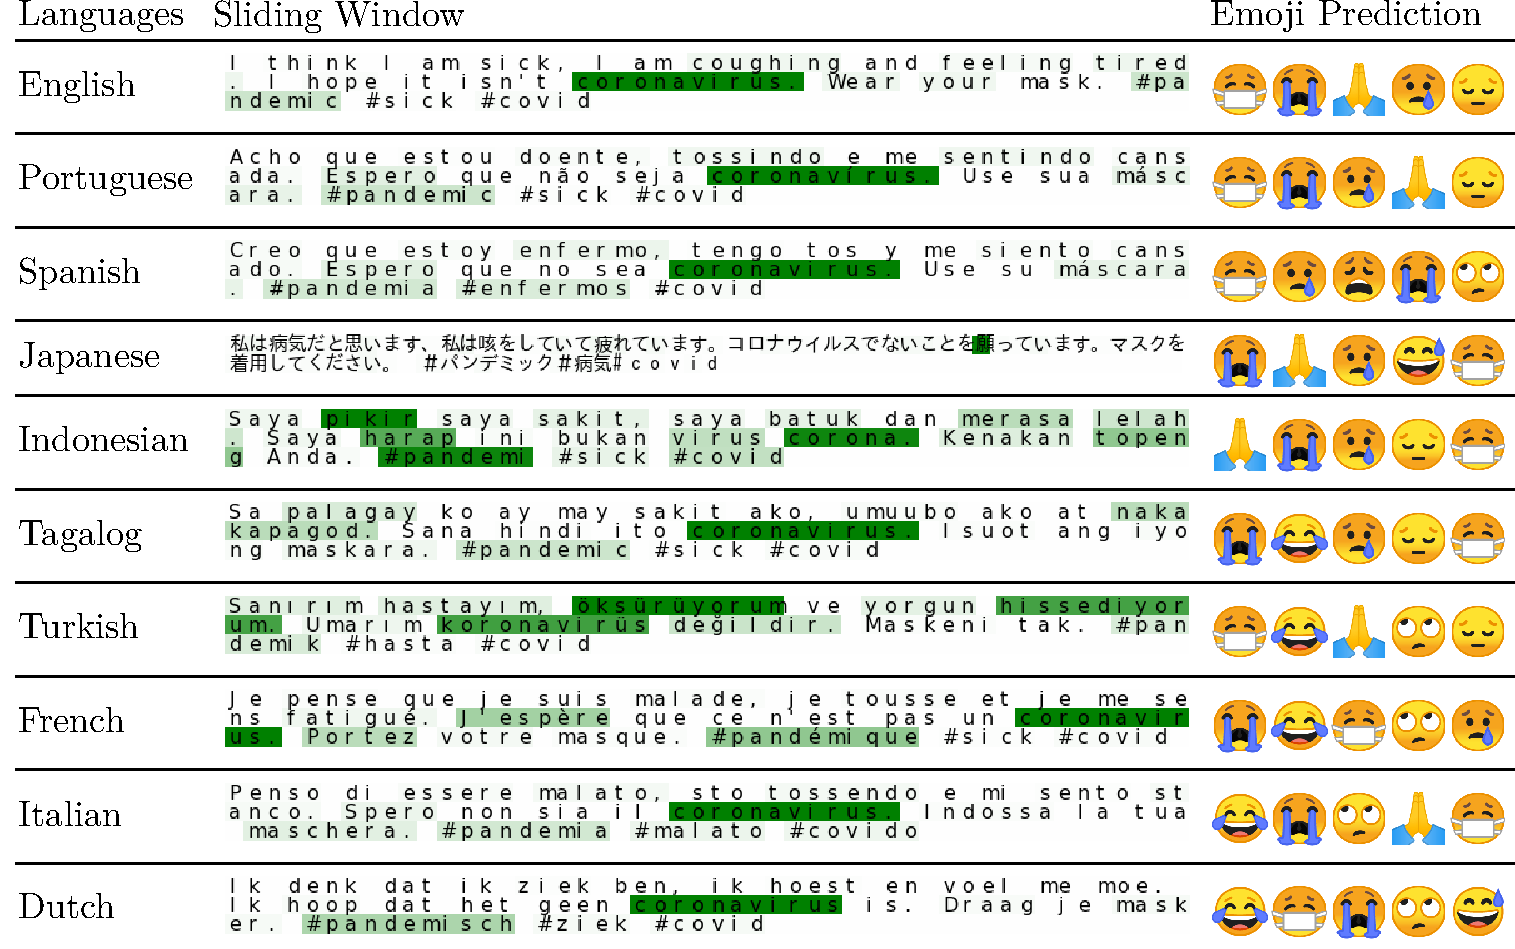
\includegraphics[width=\textwidth]{images/languages_slide_fix.pdf}
    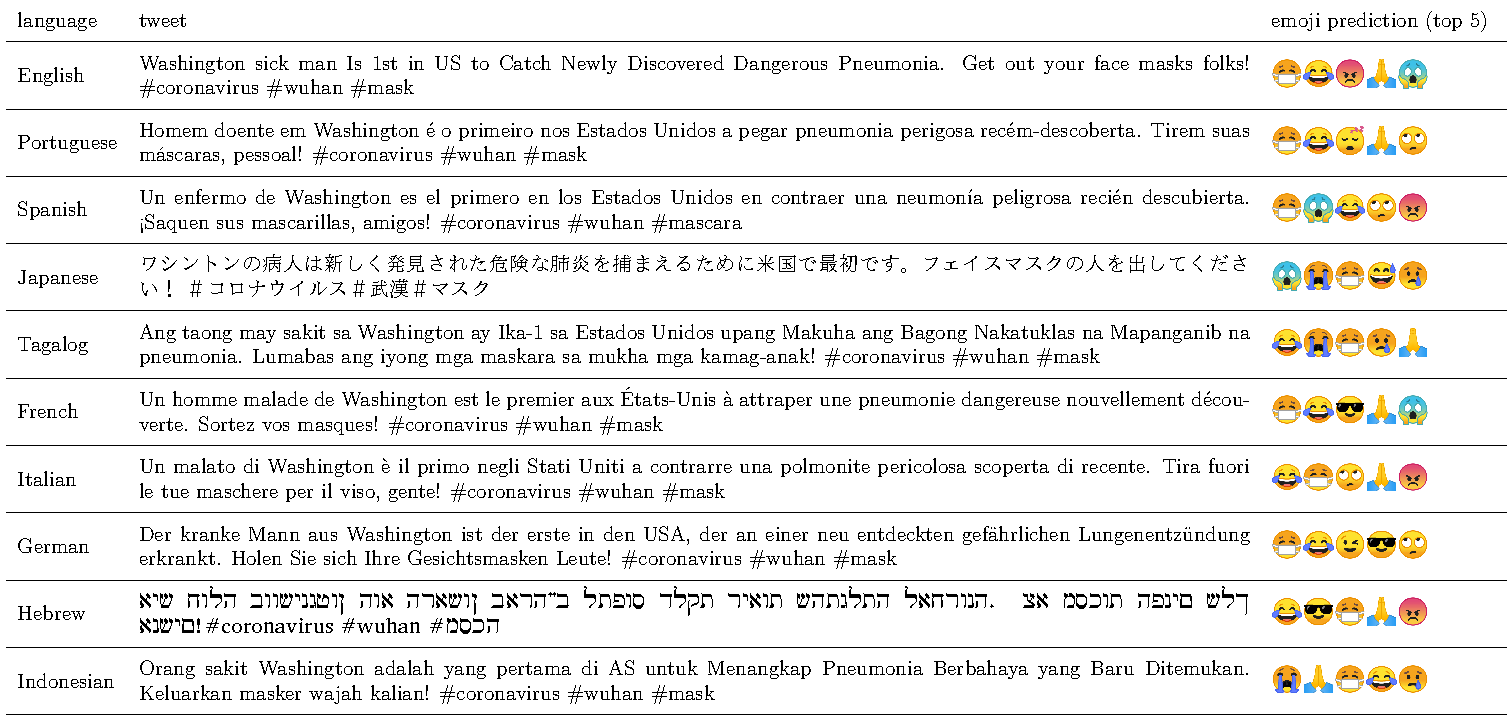
\includegraphics[height=3in]{images/table_fixed.pdf}
    \caption{
        $\bertmoji$ predicts good emojis in a wide variety of languages.
        All non-English text above was translated from the English using Google Translate.
        \fixme{
            ``Languages'' should be ``language''; ``Sliding Window'' should be ``tweet''.
        }
        \fixme{
            The font is too big.  It's bigger than the main body's text, and should be slightly smaller.  The same size as the tweets is ideal.
        }
        \fixme{
            It would be really good to have more non-Latin alphabets in here.
        }
        \fixme{
            There's not going to be room to describe the sliding window algorithm anywhere in the text,
            so I think we should take out the middle column and replace it with uncolored text.
            This will also make it easier to get good formatting in different languages.
            (I realize you spent a lot of time on the sliding window,
            but we have to do what's best for the paper,
            and that almost always means discarding some things we put a lot of work into.)
        }
        \fixme{
            The Japanese row should be the same height as all other rows.
        }
        \fixme{
            Try to fit the final figure into the 3in height I've resized it to.
            That'll be easier without the sliding window middle column.
        }
        \fixme{
            We need a brief discussion about why each language predicts different emojis.
            Ideally we would be able to argue this based on how different languages use different emojis.
            For example, is it the case that Indonesians/Japanese use the folded hand emoji more often than English tweets?
            I associate both of these countries as being particularly spiritual, and so that would make sense to me if they are using these emojis to represent prayer,
            and that would tell a very interesting story that this workshop would be interested in.
        }
        \fixme{
            The tweet text doesn't seem like something that someone is likely to actually tweet.  Rather than making up your own text, it might be useful to use a tweet that's actually in the dataset.
        }
     }
    \label{fig:prediction_top10_langs}
\end{figure}


Emojis are well known to encode the emotional content of tweets \citep{sari2014user,kralj2015sentiment,eisner2016emoji2vec,wood2016emoji,felbo2017using,shoeb2019emotag}.
%Emoji prediction is therefore a more attractive task than direct emotion prediction because of the difficulty in obtaining quality emotion labels.
%\citet{mozetivc2016multilingual} show that human annotators are incredibly difficult to coordinate in multilingual sentiment evaluation tasks.
And therefore several works have tackled the problem of predicting emojis from a tweet's text as a proxy for predicting emotion \citep{barbieri2017emojis,felbo2017using,Zhang2019}.
This prior work focuses primarily on English-language tweets.
Models submitted for the SemEval 2018 Task 2 \citep{barbieri2018semeval} are the most multilingual emoji prediction models currently published,
but this task considered only English and Spanish tweets.
Because COVID-19 is a worldwide phenomenon, however, to understand emotional responses to COVID-19, we must be able to predict emojis in all languages used on Twitter.
We therefore introduce the first highly multilingual model for emoji prediction, which we call $\bertmoji$.
Our model is based on fine-tuning the multilingual BERT model \citep{devlin2018bert},
which was trained on a dataset of 102 distinct languages.
Figure \ref{fig:prediction_top10_langs} shows the output of our model in a tweet translated into ten different languages.
%Emojis are rendered differently across different platforms, leading to translation issues \citep{miller2018see}

%Following the work of \citet{fixme1,fixme2,fixme3}, we use emojis as distant labels for emotions.
%Hand classifying text by emotions is an expensive and error prone process,
%and the largest existing datasets for this task contain only about 10,000 tweets focusing on the limited domains of video games \citep{fixme} or stock performance \citep{fixme}.

%In the times that we are facing, exploring the public's sentiment offers useful insight into how people react to situations of stress, anxiety and uncertainty. A perfect source to explore this is through Twitter's API.\cite{subasish2020} draws from tweets related to Covid19 and India and by using public available sentiment analysis tools explores the public's sentiment on a two sentiment basis (negative and positive). 
A large body of work has emerged analyzing tweets about the coronavirus.
One prominent line of research attempts to identify how misinformation about the virus spreads online \citep{kouzy2020coronavirus,sharma2020coronavirus,yang2020prevalence,elhadad2020covid,prabhakar2020informational}.
An important subcategory of this research investigates the spread of racist \citep{budhwani2020creating,schild2020go} and ageist \citep{jimenez2020coronavirus} misinformation.
Other research more similar to our own investigates the sentiment of tweets about the coronavirus.
Some of this research focuses on specific locations such as Belgium \citep{kurten2020coronavirus}, Paris \citep{saire2020study}, Poland \citep{jarynowski2020perception} or India \citep{subasish2020}.
Other research focuses on all English-language tweets \citep{rajput2020word,yin2020detecting},
and therefore consider a wider geographic area.
Our research stands out from this prior work in two important ways.
First, we consider all tweets about the coronavirus, written in all languages, sent from anywhere in the world.
This is a significantly more challenging technical problem than previous research addressed,
and it is also much more useful.
Second, we are the first paper to consider the more general emoji prediction problem rather than the sentiment prediction problem.
In sentiment prediction,
the goal is to assign a positive or negative sentiment to each tweet,
and for the coronavirus this is almost trivial---the vast majority of tweets about the coronavirus express negative sentiments.
In the emoji prediction task, however, we are able to get a more fine-tuned emotional understanding of tweets to understand why the sentiment is negative.

%college students respond differently \citep{duong2020ivory}
%map travel patterns using geotagged tweets \citep{feng2020working}

Our contributions are as follows.
In Section \ref{sec:bertmoji} we introduce the first dataset for training highly multilingual emoji prediction models, $\emoticon$.
We then use this model to train the first highly multilingual emoticon prediction model, $\bertmoji$.
Our model is open source and has an easy to use PyPi package.%
\footnote{
    URL blinded for peer review.
}
In Section \ref{sec:casestudy}, we introduce the first highly multilingual dataset of tweets about the coronavirus, called $\corona$.
To generate the dataset, we introduce a novel method combining Bing Translate and the \texttt{spacy} tokenization library \citep{spacy2}.
We then apply the $\bertmoji$ model to the $\corona$ dataset to map how Twitter users across the world have emotionally responded to a variety of COVID-19 news events.
This is the first highly multilingual emotion analysis of tweets in any language,
and the most comprehensive analysis specifically about the COVID-19 pandemic.

%%%%%%%%%%%%%%%%%%%%%%%%%%%%%%%%%%%%%%%%%%%%%%%%%%%%%%%%%%%%%%%%%%%%%%%%%%%%%%%%

\section{The $\bertmoji$ Model}
\label{sec:bertmoji}

In this section, we first present the $\emoticon$ dataset that the $\bertmoji$ model was trained on.
Then we describe our training procedure and model evaluation results.
We take particular care to ensure that the $\emoticon$ dataset is sampled from a similar distribution to the $\corona$ dataset analyzed in Section \ref{sec:casestudy} below in order to ensure that the $\bertmoji$ model will transfer well to this unlabeled dataset.
%The purpose of the $\emoticon$ dataset is to develop the emotion classifier which we will later use in our case study of coronavirus-specific tweets.
%The $\emoticon$ dataset is large, with \XXX million tweets in at least 66 languages sampled from the same distribution as our coronavirus tweets.
%Therefore, we can expect a classifier trained on the $\emoticon$ dataset to transfer well to the $\corona$ dataset.

%%%%%%%%%%%%%%%%%%%%%%%%%%%%%%%%%%%%%%%%

\subsection{The Target Emoticons}

\begin{figure}
    \centering
    \subfloat{{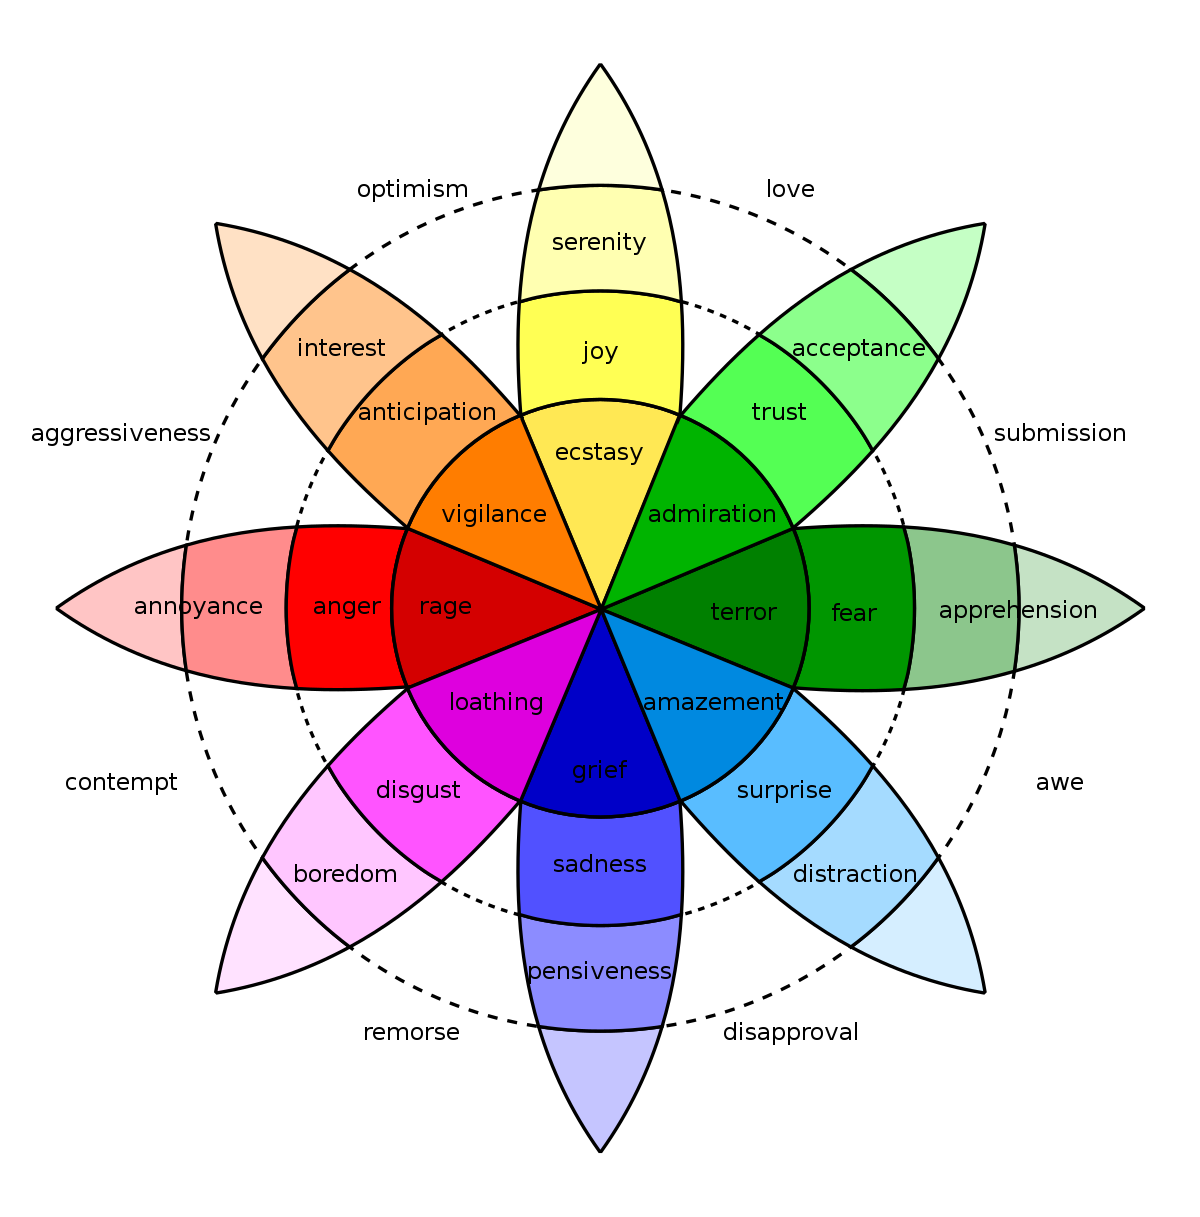
\includegraphics[scale=0.125]{images/Plutchik-wheel.png}}}%
    \label{fig:plu_wheel}
    \subfloat{{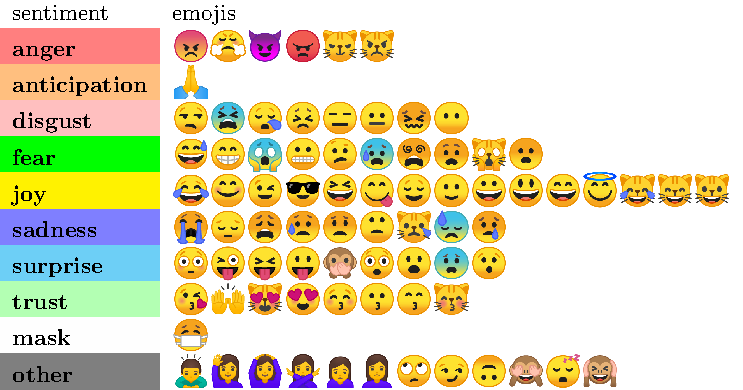
\includegraphics[scale= 0.78]{images/categories_fixed.pdf}}}%
    \caption{
        (\emph{Left}) 
        The Plutchik wheel of emotions.
        %\footnote{\url{https://en.wikipedia.org/wiki/Robert_Plutchik}}
        (\emph{Right}) 
        We have grouped the emoticons into 10 different categories:
        8 emotional categories from the Plutchnik wheel,
        1 category for the ``face with medical mask'' emoticon,
        and 1 category for all other emoticons that represent emotions that are not clearly in the Plutchik wheel.
        \fixme{
            You need a label for the emotions column.  You also need to shrink the table vertically so that it's the same exact height as the Plutchik wheel.
        }
    }
    \label{fig:Mapped_emojis}%
\end{figure}


Emojis were first added to the Unicode standard in 2010,
and the current version of the standard (12.1.0) defines 3304 different emojis \citep{unicode12}.
Prior work on emoji prediction has limited itself to predicting only a subset of the available emojis.
For example, \citet{barbieri2017emojis} consider only the 20 most commonly used emoji,
and DeepMoji \citep{felbo2017using} considers only 64 emoji.
There are two primary reasons for only considering a subset of emoji.
First, emoji-usage follows a power law distribution where the top 1\% of used emoji account for over 99\% of all emoji usage.%
\footnote{
    See \url{http://www.emojitracker.com/} for real-time stats on Twitter emoji usage.
}
There is therefore very little training data for the less popular emojis,
and so we cannot expect a classifier to have high prediction accuracy for these emoji.
Second, many emoji (e.g.\ the Greek Flag emoji \XXX) do not contain emotional information,
and so the ability to predict these emoji does not help us understand the emotional content of text.

We follow previous work and focus on predicting only a limited set of emoji.
Specifically, we focus on the original 80 emoji defined in the Unicode standard's emoticon code block (code points \texttt{0x1f600} - \texttt{0x1f650}). %\footnote{
    In common usage, the words \defn{emoji} and \defn{emoticon} are interchangeable,
    but in this paper we adopt the Unicode Standard's definitions of these terms.
    By these definitions, an \defn{emoji} is any one of 3304 pictographs that are not part of any written language,
    and an \defn{emoticon} is one of the original 80 emoji defined in the code block specified above.
%}
We limit are analysis to emoticons for three reasons.
First, they are the most commonly used emoji on twitter,
so we can expect to achieve relatively accuracy.
Second, each emoticon represents an emotion (emoticon is a portmanteau of emotion and icon).
Third, the emoticon block contains the ``face with medical mask'' emoji (
\includegraphics[height=0.8em]{images/mask_photo.png}),
which is important for our case study analyzing emotional responses to the coronavirus.

Figure \ref{fig:Mapped_emojis} shows the 80 emoticons and a mapping from these emoticons to the Plutchik wheel of emotions \citep{plutchik1991emotions}.
The Plutchik wheel is a standard psychological model for encoding emotions that has been highly influential in emotion prediction systems.
It has 8 primary emotional categories (anger, anticipation, disgust, fear, joy, sadness, surprise, and trust).
These emotions are arranged spatially so that similar emotions (e.g.\ joy, trust) appear near each other, and dissimilar emotions (e.g.\ joy, sadness) appear opposite each other.
Furthermore, each emotional category is broken down into sub-categories called ``valences'' that encode the strength of the emotion (e.g.\ ecstasy is an extreme, and serenity is a mild version of joy).

There is currently no standard mapping from emoticons onto the Plutchik wheel,
and in Figure \ref{fig:Mapped_emojis} (\emph{right}) we provide a suggested mapping.
To generate this mapping, we manually assigned each emoji to an emotion based on the description of the emoji on the website \url{emojipedia.org}.
The mapping is not perfect.
The category joy has many emoticons representing different facets of joy,
but the category anticipation has only a single emoticon.
We emphasize that our $\bertmoji$ model will predict raw emoticons directly;
we present the Plutchnik wheel emotions only as a more easily-digestible summary of these emoticons.

%We used NVidia's \texttt{sentiment-discovery} library to provide a preliminary sentiment analysis of the $\corona$ dataset,
%and the results are shown in Figure \ref{fig:nvidia-sentiment}.
%The results are not very informative, however, because NVidia's model was trained on a small set of English-language tweets (about 16 thousand) about video games,
%and there is little reason to believe that this domain would transfer well to the coronavirus domain.

%%%%%%%%%%%%%%%%%%%%%%%%%%%%%%%%%%%%%%%%

\subsection{The $\emoticon$ Dataset}

\begin{figure}%
    \centering
    \subfloat{{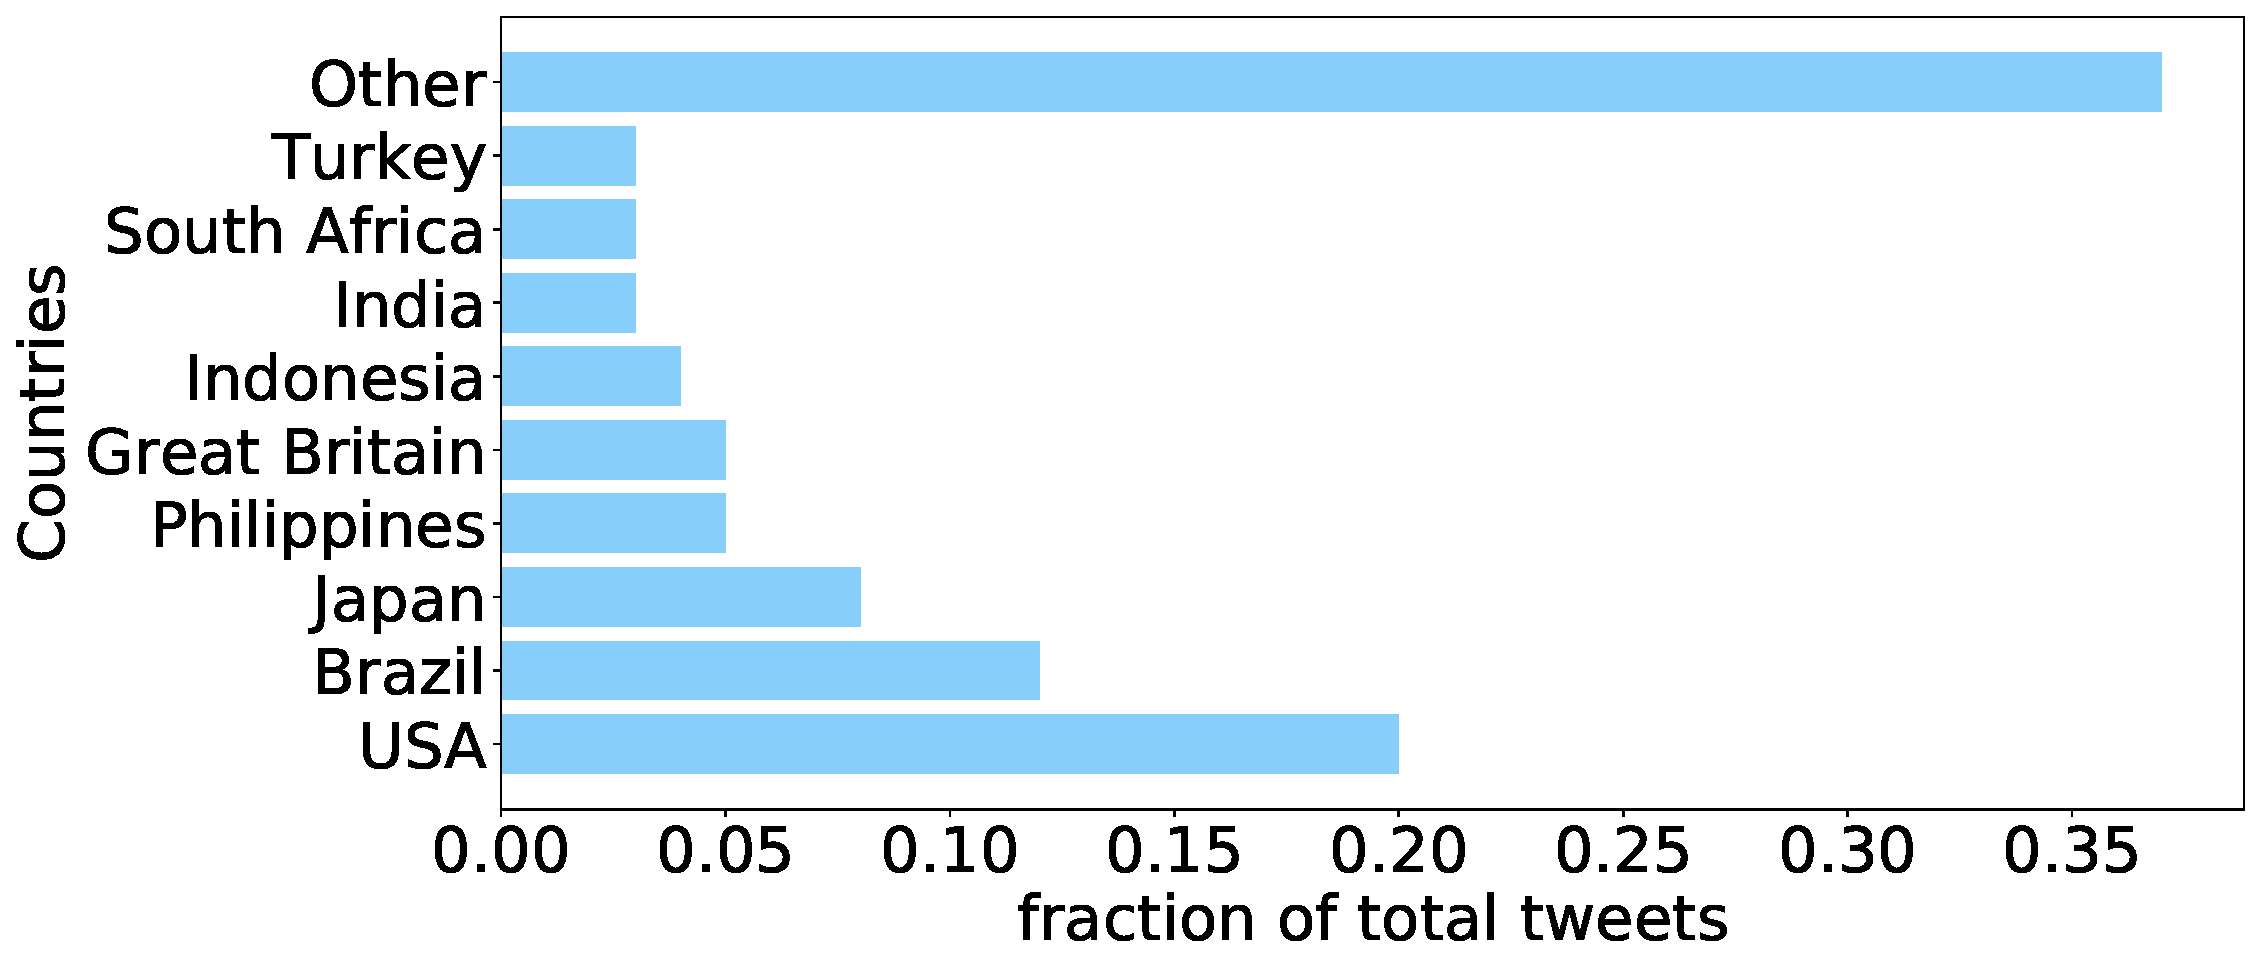
\includegraphics[scale=0.21]{images/dis_country_fixed.eps}}}%
    \label{adsad}
    \subfloat{{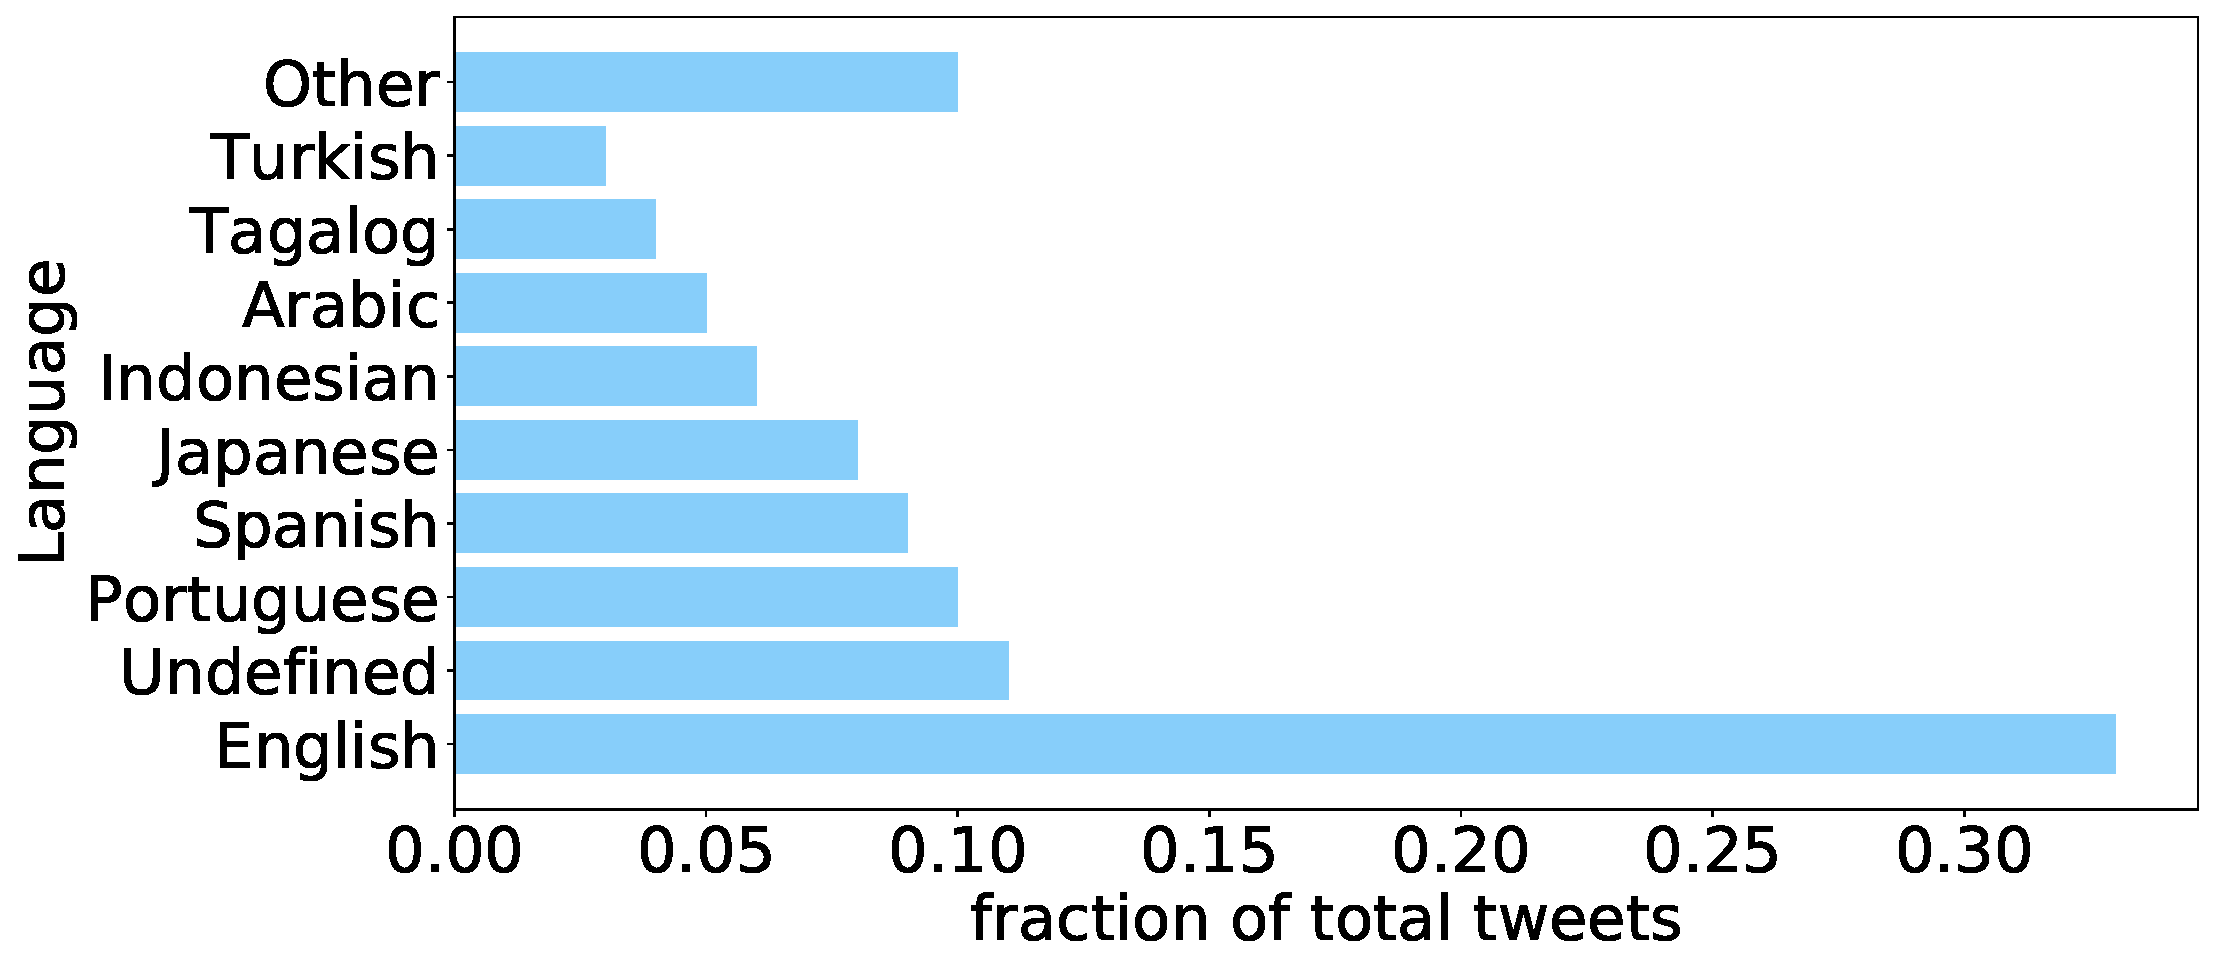
\includegraphics[scale =0.21]{images/dis_lang_fix.eps} }}%
    \caption{ 
        Stats on the most common countries of origin (\emph{left}) and languages (\emph{right}) for tweets in the $\emoticon$ dataset.
        Languages are determined using Twitter's API, which has official support for \XXX languages.
        It is known, however, that more than 100 language are actively used on Twitter \citep{fixme},
        and our $\bertmoji$ model supports all of these languages.
        All prior work on emoji prediction has focused tweets in either only English,
        or just English and a single other language.
        \fixme{
            The y-axis is not a percent, it is a fraction;
            plus, you always need to say what something is a fraction/percent of.
            Change the label to ``fraction of total tweets''.
        }
        \fixme{
            Your x-tic labels are very difficult to read.
            For example, your label for ``South Africa'' touches the Turkey bar but doesn't touch the ``South Africa'' bar.
            This needs to be fixed by either: rotating everything so that the bars are horizontal (best option),
            or making the x-tic labels vertical.
        }
    }%
    \label{fig:stats:countrylang}%
\end{figure}

%The $\emoticon$ dataset is specially designed for training the $\bertmoji$ model on tweets related to coronavirus.
The $\emoticon$ dataset is designed for training a classifier that takes as input a tweet and outputs an emoticon that represents the emotion of the tweet.
To generate the $\emoticon$ dataset, 
we collected all geolocated%
\footnote{
Twitter users can adjust their privacy settings to include different amounts of geolocation metadata.
In particular, they can include the exact GPS coordinate that a tweet was sent from,
an approximate location (for example, the city that the tweet was sent from),
or no location information at all.
We say that a tweet is \defn{geolocated} if any of this metadata is included about the tweet.
Approximately 1\% of all tweets are geolocated.
} 
tweets sent over the six month period between January and June, 2020.
Approximately 400 million tweets meet this criteria.
Then we filtered these tweets so that only tweets containing one of our 80 target emoticons were included,
and any retweets were removed.
In total, the $\emoticon$ dataset contains 64.2 million tweets sent by 4.2 million users.
The tweets are written in 66 different languages and were sent from 246 different countries.
Figure \ref{fig:stats:countrylang} shows the total number of tweets per language,
and Figure \ref{fig:stats:emoticon} shows the frequency of each emoticon in the dataset.

We preprocess each tweet by replacing all user mentions with a special token \texttt{<mention>} and all URLs with a special token \texttt{<url>} and deleting all emojis.
We decided to keep all hashtags because hashtags can contain potentially valuable emotional content useful for emoticon prediction.
Finally, we delete all emoticons from the tweet,
and use the emoticons as the tweet's classification label.
Most tweets have only a single emoticon label, but some tweets have multiple emoticons.
This is a problem because standard multi-class classification techniques require only a single label per data point.
We address the issue by following the procedure established by \cite{100_million_tweets}:
If a tweet has multiple emoticons,
then we duplicate it in the training data once for each emoticon,
with each instance being labeled by a single one of the emoticons.
%where for each unique emoji in a tweet, we have a separate tweet with that emoji as a label. 
%For tweets containing repetitions of the same emoji; we only save one instance of it.
%Finally, each tweet is labelled with the emojis that were deleted from the tweet.

\begin{figure}
    \centering
    %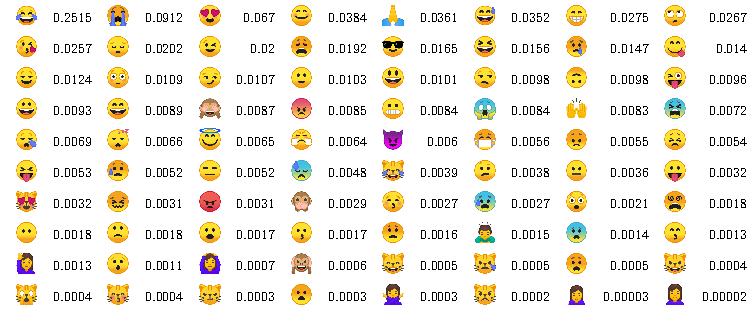
\includegraphics[scale = 1.2]{images/emojitable.pdf}
    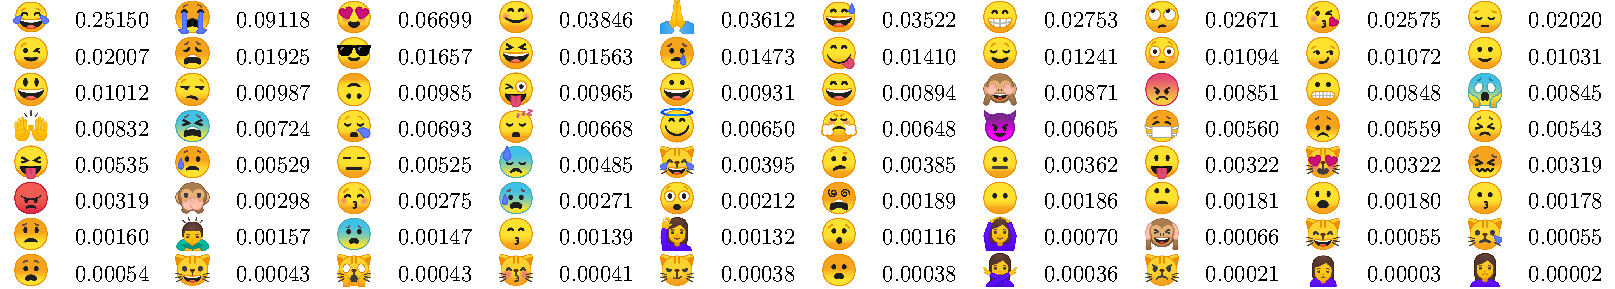
\includegraphics[width = \textwidth,height=1.3in]{images/emoji_table_fix.pdf}
    \caption{
        The emoji distribution of the $\emoticon$ dataset.
        \fixme{All numbers must have either 4 or 5 decimals.  For example 0.02 should be 0.0200}
        \fixme{The figure needs to take up max 2 inches vertically, but ideally it would be more like 1.5}
    } 
    \label{fig:stats:emoticon}
\end{figure}

We carefully split the $\emoticon$ dataset into training, validation, and test sets ensuring that no user is present in all three sets in order to prevent data leakage.
In particular we assign 80\% of users to the training set, 10\% to the validation set, and 10\% to the test set.
The tweets contained in each set are then the tweets sent by each of the users in the set.

%%%%%%%%%%%%%%%%%%%%%%%%%%%%%%%%%%%%%%%%

\subsection{Training Protocol}

Our $\bertmoji$ model is the multilingual BERT model \citep{devlin2018bert} fine-tuned on the $\emoticon$ dataset.
The multilingual BERT model is a popular model for fine-tuning because it achieves state-of-the-art performance on a wide variety of natural language tasks.
It was trained on data from 102 distinct languages,
and the language of each training sample need not be known for either training or inference.
Followup research has shown that the multilingual BERT model has language-independent internal representations that allow it to encode information from languages it has not seen during training time \citep{pires2019multilingual,wu2019emerging}.
\citet{feng2020language} recently released a more advanced version of the multilingual BERT model that achieves better performance on standard NLP tasks and uses 109 training languages.
We would expect better performance on our emoticon-prediction task using this more advanced multilingual BERT model,
but we did not use this model because all of our experiments were completed before this model was publicly released.

We followed a two step fine-tuning procedure.
First, we trained only the last layer of the model,
generating a model we call $\bertmojill$.
Then, we trained the all parameters to generate the $\bertmoji$ model,
warm starting from $\bertmojill$.
We used the validation set to select optimal hyperparameters for both models.
$\bertmojill$ was trained using Adam \citep{kingma2014adam} with a learning rate of $10^{-4}$,
and $\bertmoji$ was trained using Adam with a learning rate of $10^{-5}$.
Both models used a batch size of 64.
A single epoch on the $\emoticon$ dataset took approximately 6 days to run on one NVidia GeForce RTX 2080 GPU.
We trained both models on a single epoch, but found that the model converged before the epoch was finished.
%
%We fine-tuned this pre-trained model to generate two models. 
%The first one only trained the last layer of the model, while the second one trained all the layers.
%We followed the Train-Validation-Test split procedure, where 1 epoch took approximately 6 days to run on one Nvidia GeForce RTX 2080 graphics card.
%The hyper-parameters with which we achieved the highest accuracies are the following. 
%When training the last layer of the model we used: a learning-rate of 1e-04, Adam optimizer and gradient clipping. 
%While training all the layers of the model we had: a learning-rate of 1e-05, Adam optimizer and gradient clipping. 
%Both models were warm-started from previous runs and the batch size used was 64.

%BERT is a new language representation model, which is aimed in pretraining deep bidirectional representations from unlabeled text by jointly conditioning on both left and right context in all layers.
%Therefore, the pre-trained model can be easily fine-tuned by adding another output layer.
%One of the reasons why we picked BERT is due to its performance on the General Language Understanding Evaluation (GLUE) \cite{} benchmark.
%It is comprised of nine language understanding tasks, assembled from a diverse dataset which includes insight into model performance with respect to a wide range of linguistic phenomena.
%At the time of writing, BERT and its variations hold a number of top achieving scores in the GLUE leader-board \ref{leaderboard}.   

\begin{figure}
    \centering
    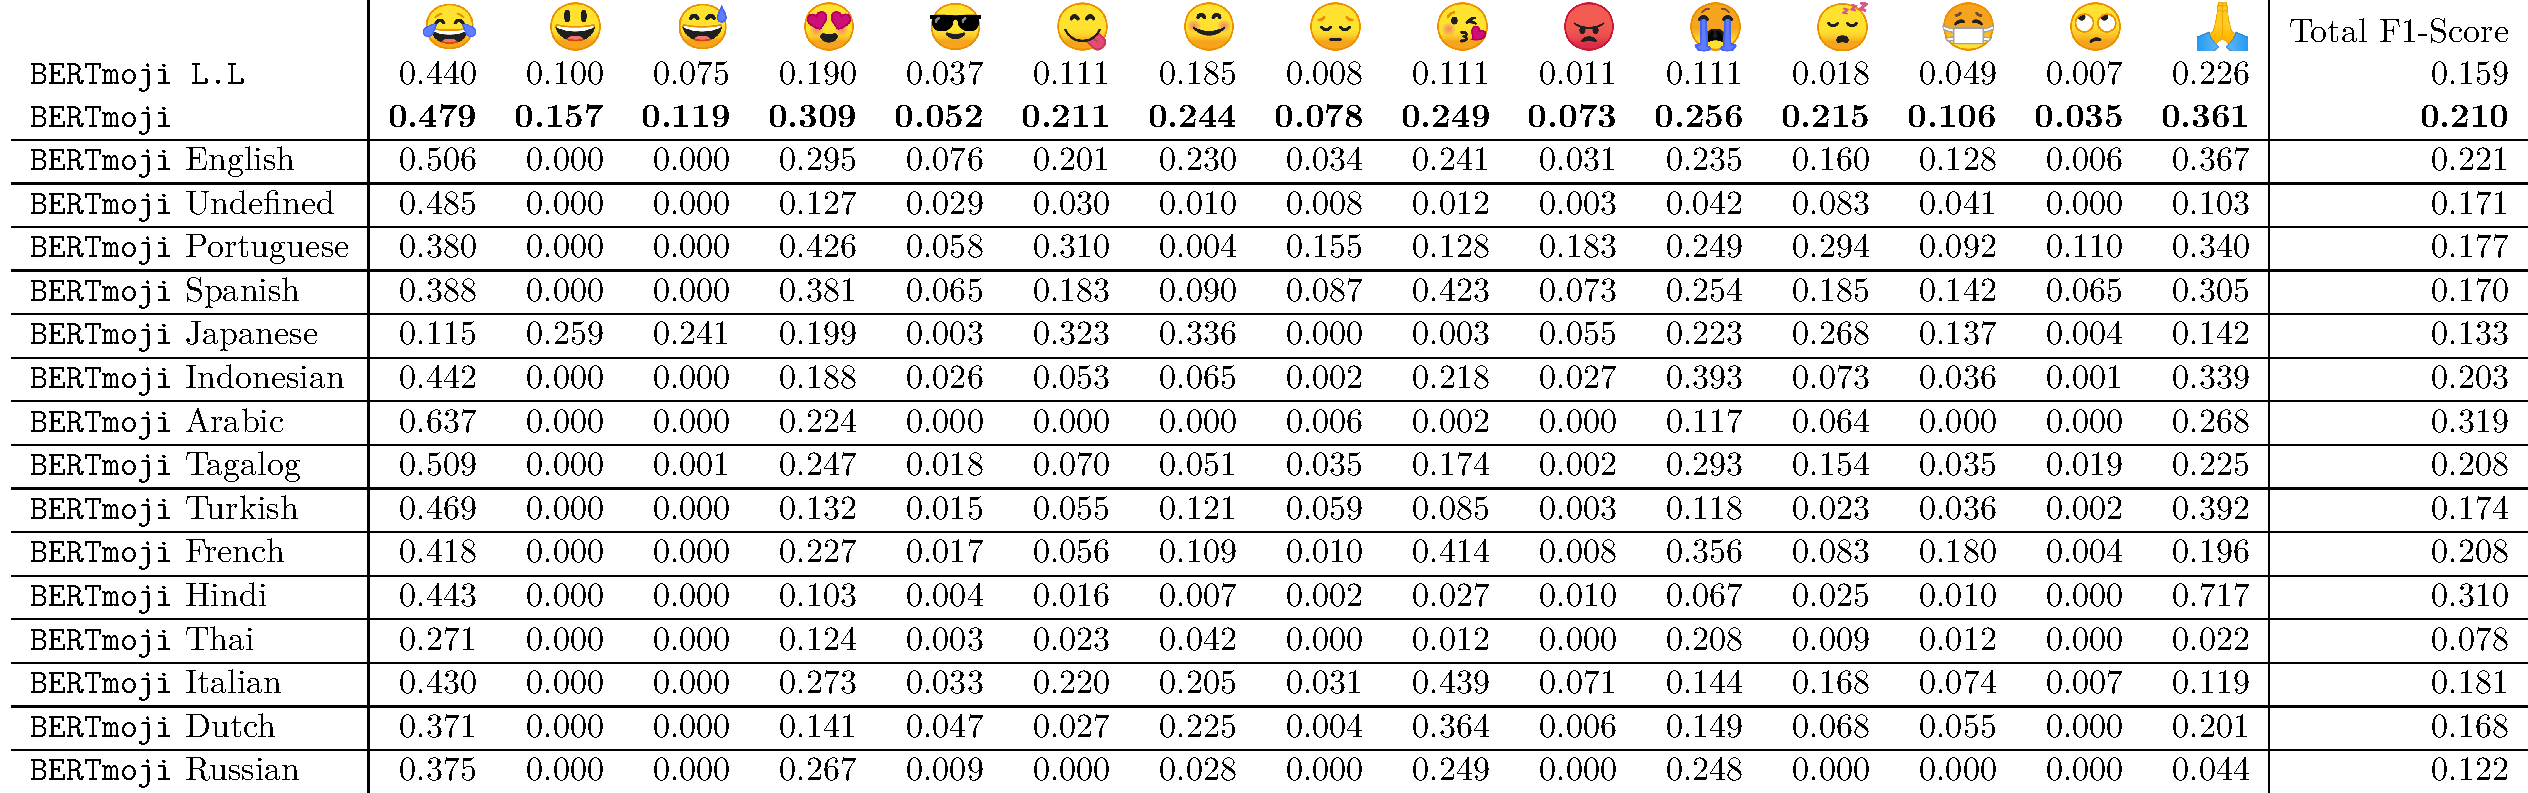
\includegraphics[width=\textwidth]{images/f1_score_table_fix.pdf}
    \caption{
        F1 scores of the $\bertmojill$ and $\bertmoji$ model on 15 selected emojis. Included also are the F1-score language breakdown. (The total is this the sum of averages, kind of showing how we go an f1 score of 21\%).
        \fixme{This is the 2nd most important figure of your paper (after the figure with all the examples), and right now it's ugly and hard to read.  This figure needs some serious cosmetic work.  If you need ideas, then let me know and I'll draw you by hand some ideas.  In the future, if you make all your tables in latex, then collaborators can easily edit them to provide suggestions (and they'll look much nicer!), but since it's just a pdf file, I can't do that.}
    }
    \label{fig:tweets_per_day}
\end{figure}

%%%%%%%%%%%%%%%%%%%%%%%%%%%%%%%%%%%%%%%%

\subsection{Model Evaluation}

We now present the results of the models. We used the scikit-learn \cite{} library, to classify our models.
We executed 2 classification for the two models. Initially we measured the f1-scores for all 80 emoji categories.
The last-layer model had an F1-score of 15.89\% while the other one achieved an F1-score of 20.97\%. 
Afterwards, we performed the classification on the top-15, F1-score achieving emojis. 
Those emojis comprised about 70 percent of the dataset.
The results were the F1-scores of 24.07\% and 31.77\% accordingly.
All the F1-scores are calculated via weighted average. Figure 3,4 presents more detailed analysis of the results.
While f1-scores vary for different emojis and languages,
both figures highlight that  $\bertmoji$ outperforms $\bertmojill$. 

We now precede in testing $\bertmoji$ ability to predict emojis for different languages.
We decided on picking an English sentence that expressed emotions and could possibly appear in twitter,
we then translated from English to the other nine languages from Figure 2 using Google Translate.
The sentence was: "Thinking about all the things I didn't do today, ok bed time ... \#tired \#sleep."
In addition, we also applied the sliding window algorithm to the translated sentences,
in order to observe which words were more significant for the $\bertmoji$ across the translations.
The results are shown in Figure 6. 

%%%%%%%%%%%%%%%%%%%%%%%%%%%%%%%%%%%%%%%%%%%%%%%%%%%%%%%%%%%%%%%%%%%%%%%%%%%%%%%%

\section{Coronavirus Case Study}
\label{sec:casestudy}

We now apply the $\bertmoji$ model to understand the emotional response of Twitter users to news about the coronavirus.
We first introduce our $\corona$ dataset,
then we present an analysis of this dataset.

\subsection{The $\corona$ Dataset}

%Twitter has released the COVID-19 stream\footnote{\url{https://developer.twitter.com/en/docs/labs/covid19-stream/overview}}
The goal of the $\corona$ dataset is to include any geolocated tweet that references the coronavirus in any language.
%There are many alternative twitter datasets available about the coronavirus.
%The most popular and comprehensive data set is due to \citet{chen2020tracking}. 
%They began tracking tweets in January 2020,
%and they consider a tweet to be about the coronavirus if it contains any of 64 keywords related to the coronavirus.
%These keywords include both individual words like ``coronavirus'' and commonly used hashtags like ``stayathome''.
%All but two of these search terms are English.%
%\footnote{The non-English terms are ``koronavirus'' and ``pandemie''.}
%Many languages
%%코로나 바이러스
%
We use a relatively complicated process to extract these tweets in order to ensure maximum recall and precision in a wide range of languages.
Our procedure is:
\begin{enumerate}
\item
We generated a list of \XXX English-language search terms related to the coronavirus,
such as \texttt{coronavirus}, \texttt{covid19}, \texttt{wuhan} and \texttt{lockdown}.
We then used Bing's translation API to translate each of these terms into the 72 languages supported by Bing translate.
%Table \ref{table:search_terms} in the supplemental material contains the full list of search terms in English and selected translations.
\item
We used Python's \texttt{spacy} library \citep{spacy2} to tokenize and lemmatize each of the \XXX million tweets in the full dataset.
\texttt{spacy} supports this process in 58 different languages,
and for each tweet we used the appropriate \texttt{spacy} module for the language specified in the tweet's metadata.
\item
Finally, the $\corona$ dataset is constructed as the set of all tweets whose lemmatized text contains any of the search terms from the tweet's language or English.
We include both languages in this filtering step because it is common for non-English tweets to use English words like \texttt{coronavirus} when referencing the virus.
\end{enumerate}
\fixme{Table \ref{table:lang} shows the 54 languages that are supported by all 3 services along with the total number of tweets in each language.}
%Figure \ref{fig:tweets_per_day_sent} provides a summary of the number of tweets per day and Figure \ref{fig:corona:spatial} shows the spatial distribution of the tweets.

\begin{table}
    \centering
    \includegraphics[height=1in]{example-image-a}
    \caption{
        Language stats.
        \fixme{Ideally we would add this table, but if you don't have time we can take it out (or maybe I'll have time to create it).}
    }
    \label{table:lang}
\end{table}

\begin{figure}
    \centering
    \includegraphics[height=0.6in,width =\textwidth]{images/true_pred_fixed.pdf}
    \caption{
        The true stacked bar presents the actual Plutchik wheel's mapped responses from the $\corona$ dataset while the predicted stacked bar graph presents the predicted emoji responses mapped to the Plutchik wheel following Figure  \ref{fig:Mapped_emojis} 
        \fixme{The labels should not be rotated.}
        \fixme{The font should be the same for all text in the figure, and much larger for the text on the top.}
        \fixme{
            Those are not percentages on top, but fractions.
            The label should tell the reader what they are fractions of.
            A better label would be ``fraction of the dataset''.
        }
        \fixme{
            You need a key here somewhere to know what each color represents.
            It's not enough to say look at Figure \ref{fig:Mapped_emojis} for a key.
        }
        \fixme{
            Shrink the height of this bar as much as possible so that the text is still readable.
            We're going to need every bit of space possible.
        }
    }
    \label{fig:actual vs pred}
\end{figure}


The other significant dataset of coronavirus related tweets is due to \citet{chen2020tracking}.
There are two main differences between our dataset and theirs.
First, we only include geolocated tweets,
whereas they include non-geolocated tweets as well.
This results in their dataset being about fifty times larger than ours,
with about 250 million tweets over the same time period.
Because their data is not geolocated, however, it is not suitable for understanding how different countries have reacted emotionally to the coronavirus.
The second difference is that our dataset uses a more advanced language-aware filtering method.
They only search for tweets that contain English keywords.
Most languages, however, have few words in common with English,
and non-Latin based languages frequently do not even use the word ``coronavirus'' to describe the virus.
Chinese tweets, for example, commonly refer to the coronavirus with the string
\begin{CJK}{UTF8}{gbsn}
病毒
\end{CJK},
and Chinese-language tweets containing this string will get included in our dataset but not in their dataset.
As a result of this more advanced processing, the fraction of non-English tweets is much larger in our dataset than theirs (\XXX versus 38\%).
Capturing as many non-English tweets as possible about the coronavirus is important for ensuring that our analysis is not unfairly skewed towards English-speaking countries.
%Again, this improves our multicultural analysis in Section \ref{sec:}.

%Importantly, duplicate tweets are included in the $\corona$ dataset,
%but they are not included in the $\emoticon$ dataset.
%This is because of the purpose of the $\emoticon$ dataset. 
%We aimed to apply our $\bertmoji$ to this dataset,
%which is something with free user input where our training data is not fully representative of the eventual data our model will be applied to.
%Therefore this limits our abilities to make assumptions and could possibly inflate our sense of model efficacy.
%On the other hand when dealing with the $\corona$ dataset,
%duplicate inputs result in some distribution on our outputs.
%Since we want to map out the public's emotional response to the coronavirus, it is important 
%for those distributions to be maintained.

%%%%%%%%%%%%%%%%%%%%%%%%%%%%%%%%%%%%%%%%

\subsection{Results}

\fixme{I'll add a bit more here based on how much space we have available.}

\begin{figure}
    \centering
    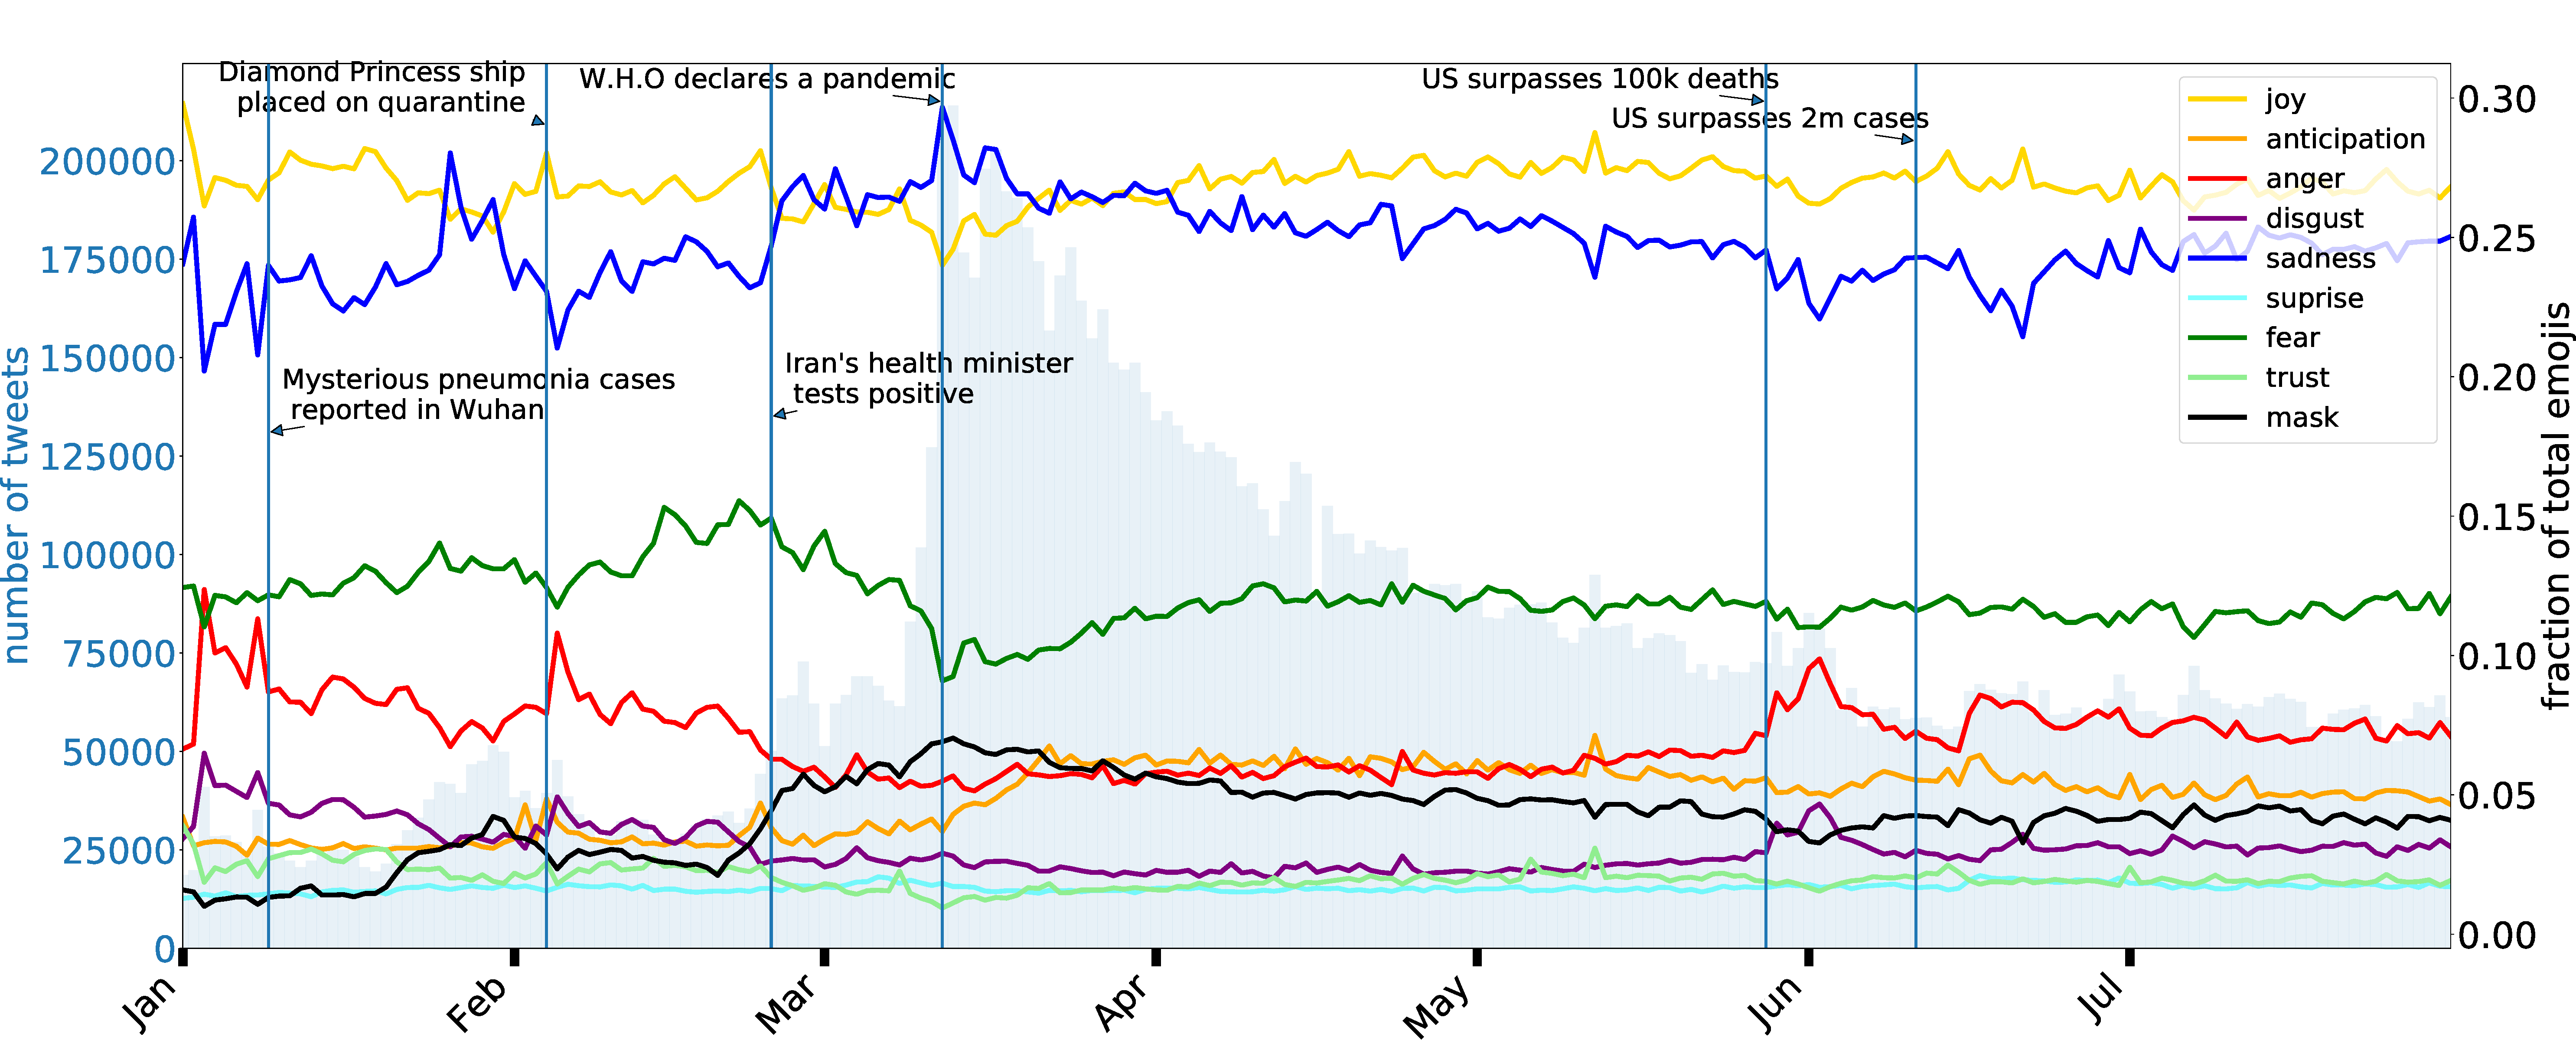
\includegraphics[width=\textwidth,height=2.5in]{images/twitter_graph_fixed.pdf}
    \caption{
        The emotional content of tweets in the $\corona$ dataset changes over time and reacts to major news events.
        The shaded bar plot in the background shows the total number of tweets in the $\corona$ dataset sent on a particular day,
        and the colored line charts show the fraction of tweets in a particular day that correspond to each emotion on the Plutchik wheel or the mast emoji.
        We can see clear emotional reactions to the news events labelled with vertical lines.
        %For example, when WHO declared a pandemic on $\XXX$, we can see a peak in the amount of 
        \fixme{The fonts are way too small.}
        \fixme{The month names should not be rotated, and there should be a tic on the x-axis indicating the first of each month.}
        \fixme{
            Do we have any reason to believe that uptick in anger/disgust and downtick in sadness/fear in February is due to the Diamond Princess being in quarantine?
        }
        \fixme{
            Can we find out what's going on at mid-January, late February, and mid-June that's causing the changes in emotion?
            Adding labels for those events would make the figure quite a bit stronger.
        }
    }
    \label{fig:tweets_per_day_sent}
\end{figure}

Only $\XXX$ percent of tweets in the $\corona$ dataset contain an emoticon.
We used the $\bertmoji$ model to label the remaining tweets.

Our main result is shown in Figure \ref{fig:tweets_per_day_sent}.
For each day, we calculate the fraction of tweets that represent each emotion from the Plutchik wheel (see Figure \ref{fig:Mapped_emojis}),
and we can observe a strong correlation between the emotional content of tweets and important COVID-19 news.
On March $\XXX$, the World Health Organization (WHO) declared COVID-19 a worldwide pandemic.
At the same time, we can see a large spike in tweets about the coronavirus,
and in particular we see an increase in sadness and a decrease in joy.
Since sadness and joy are at opposite ends of the Plutchik wheel of emotions,
it makes sense that a rise in one would cause a fall in the other.
Surprisingly, however, we also see a decrease in the fraction of fear related tweets.
We propose two possible mechanisms for this decrease.
%The first mechanism is the fact that

%Due to the fact that emojis such as crying-face with tears, dominate the $\emoticon$ dataset,
%we allow the model to predict up to 5 unique emojis for one tweet, to promote more diversity among our results.
%This way, the results can be more meaningful. Further research, can include a more balanced $\emoticon$ dataset.
%We collect the 5 predicted emojis, and after mapping them to the correct sentiment category, we calculate their 
%percent out of the total number of emojis predicted for that day. 
%In order to understand the results we collected all the emojis from the tweets in the $\corona$ and mapped them to the categories in Figure \ref{fig:Mapped_emojis}.  

\section{Conclusion}

We introduced the first model for highly multilingual emotion analysis,
and applied this model to understanding how Twitter responded emotionally to news events about the coronavirus.
It's our belief that the $\bertmoji$ model can be used to analyze the emotions of text in other context,
and we make our model available in an easy to use Python package to facilitate this process.

%{ \color{blue} \lipsum[1-2] }

%%%%%%%%%%%%%%%%%%%%%%%%%%%%%%%%%%%%%%%%%%%%%%%%%%%%%%%%%%%%%%%%%%%%%%%%%%%%%%%%
%%%%%%%%%%%%%%%%%%%%%%%%%%%%%%%%%%%%%%%%%%%%%%%%%%%%%%%%%%%%%%%%%%%%%%%%%%%%%%%%
%%%%%%%%%%%%%%%%%%%%%%%%%%%%%%%%%%%%%%%%%%%%%%%%%%%%%%%%%%%%%%%%%%%%%%%%%%%%%%%%
%%%%%%%%%%%%%%%%%%%%%%%%%%%%%%%%%%%%%%%%%%%%%%%%%%%%%%%%%%%%%%%%%%%%%%%%%%%%%%%%
%%%%%%%%%%%%%%%%%%%%%%%%%%%%%%%%%%%%%%%%%%%%%%%%%%%%%%%%%%%%%%%%%%%%%%%%%%%%%%%%

%\bibliographystyle{coling}
\bibliographystyle{plainnat}
\bibliography{main}

\end{document}
